\subsection{VDCU(Vehicle Dynamics Control Unit)}
VDCU is a vehicle dynamics control unit. It manipulates torque request from driver pedal to calculate final torque for all 4 motors. The calculated torque never exceed driver request as driver request is processed as torque limitation Traction control can only decrease the total amount of requested torque.

\subsubsection{Description}
Board uses only LV and 2x CAN bus.\\
HW :
\begin{itemize}
\item Texas Instruments C2000 Delfino F28377 MCU\\
\item 5 V can transceiver TJA1049\\
\end{itemize}

\noindent SW:\\
Board is programmed using simulink embedded coder. Advantage is that we can use our developed code for IPG Carmaker simulation (MIL) directly into our formula. VDCU uses pedal position, inertial measurement, steering wheel sensor, wheel speed sensor and motor encoders to manipulate the torque. Measurements are fed into our yaw rate control system. Output is a torque vector fed to torque vectoring algorithm that calculates the torque distribution for all wheels The resultant torque for individual wheels is lowered by traction control algorithm if needed and fed to motors.

\begin{figure}[H]
	\centering
	\includegraphics[width=\textwidth]{./img/VDCU-pcb.jpg}
	\caption{PCB of VDCU.}
	\label{fig:VDCU-pcb}
\end{figure}

\subsubsection{Wiring, cables}
Module is connected using headers to ECUB.

\subsubsection{Position in car}
Inside ECUB box.

\subsection{LV part 2}
\todo[inline]{Describe those parts here which interfere or influence the tractive system, for example a controlling unit that measures wheel speeds and steering angle and calculates a target torque for each motor or a DC/DC-Converter providing power for the LV-system from the HV-system, etc.}
\todo[inline]{wheel speed - ECUB}
\todo[inline]{steering wh. angle - ECUP}

\subsubsection {DC/DC-Converters for the car GLVS and ACP cooling fans}
Two additional DC/DC converters are present in the ACP, within the ECUA. The first DC/DC supplies the car GLVS with 24 V. The second one is the power supply for ACP cooling fans. Both DC/DC converters are of the same type, CINCON, CFB600-300S24. This type converter is an isolated type, 3000 VAC min., as per the device datasheet. (\ref{app:glvs_dcdc}). The GLVS is therefore safely isolated from the HV, same applies for the ACP cooling system, that is also isolated from the car GLVS, due to having a separate DC/DC converter.

\subsubsection{Description}

\begin{figure}[H]
	\centering
	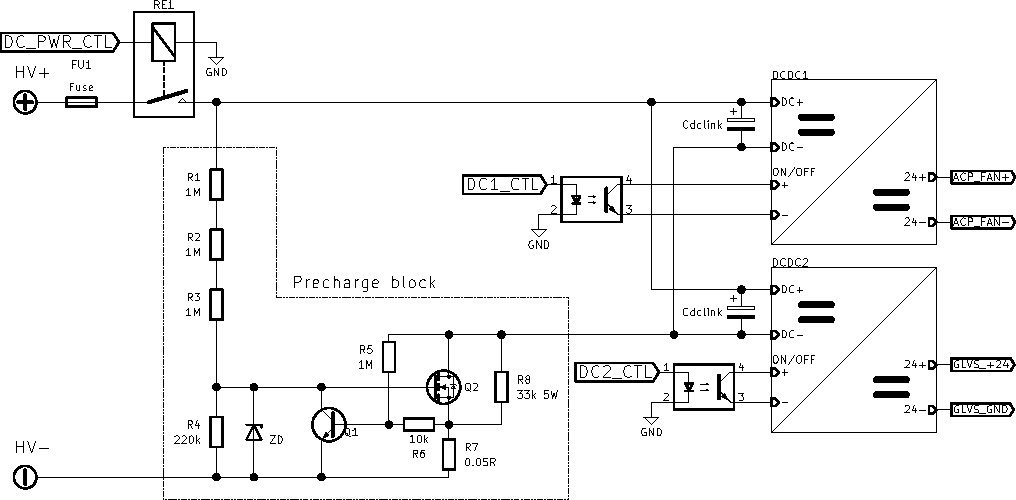
\includegraphics[width=\textwidth,clip]{./img/ECUA_DCDC_PRECHARGE.pdf}
	\caption{DC/DC pre-charge circuit and switching schematic.}
	\label{fig:precharge_dcdc_sch}
\end{figure}

Overall block diagram of the DC/DC circuitry is in \ref{fig:precharge_dcdc_sch}. Both DC/DC converters DCDC$_1$ and DCDC$_2$ share the same HV supply circuit, fused by fuse FU$_1$. Both DC/DC converters are isolated from the ACP HV using relay RE$_1$. As additional DC link capacitors $C_{dclink}$ are required for the converters on the input HV side, a separate pre-charge circuit utilizing relay RE$_2$ and NTC thermistor RT$_1$ is also required (\ref{app:ntc_datasheet}). 
All relays are the same type, Finder 40.52 (\ref{app:precharge_relay_datasheet}), two contacts always series connected to enhance the DC breaking capacity. Both DC/DC converters are always switched off first using their dedicated ON/OFF inputs, therefore there is no requirement for full DC current breaking capacity for the relays RE$_1$ and RE$_2$. In case of failure of one of the DC/DC converters, a fuse FU$_1$ will act to protect against further damage.

\paragraph{Failure behavior and response}
\begin{itemize}
	\item A failure of any of the two relays RE$_1$ or RE$_2$ either in open or close state should not present a safety risk for the driver of the car or staff members manipulating with the ACP as a whole unit. 
	Worst case is the pre-charge relay failing closed, resulting in full inrush current flowing at RE$_1$ closing, resulting in possibly blowing the input fuse FU$_1$. Pre-charge relay RE$_2$ failing closed state does not limit the functionality of the circuit, as the NTC thermistor RT1 can take over the full operating current of both DC/DC converters.
	\item Failure of the RE$_1$ relay in closed position only presents risk of draining the ACP charge away because of the stand-by currents of both DC/DC converters. As the stand-by current of both DC/DC converters is negligible and the state of the HV circuitry of the DC/DC converters is monitored using the measurement circuitry block, the ECUA maintenance members can be notified of the failure, using the car diagnostics over the CAN bus.
	\item Failure of the RE$_1$ relay in closed position only presents risk of draining the ACP charge away because of the stand-by currents of both DC/DC converters. As the stand-by current of both DC/DC converters is negligible and the state of the HV circuitry of the DC/DC converters is monitored using the measurement circuitry block, the ECUA maintenance members can be notified of the failure, using the car diagnostics over the CAN bus. 
	\item RE$_1$ failing open presents no risk, as none of the DC/DC converters will work (ACP cooling failure, GLVS supply failure) and both the car would not be able to turn on properly and transition to the TS ON state.
	The measurement block of the DC/DC converter HV input side is supplied using a small auxiliary isolated DC/DC converter (DATASHEET). Signalling from the measurement block to the GLVS control side of the car is done utilizing a combination of digital signal isolator, Silabs Si8600 series (datasheet).
\end{itemize}


Both DC/DC converters DCDC$_1$ and DCDC$_2$ are fully protected against continuous overload or short circuit condition on their output, as specified in the device datasheet. Additional isolated current sense circuits are used on both converters, using a hall effect sensor, type ACS712 from Allegro \ref{app:acs712_datasheet}. These sensors are only informative, used only for diagnostic purposes to measure current consumption from the car's GLVS system and ACP cooling.
\todo[inline]{taky do seznamu failu?}

\subsubsection{Wiring, cables}
Describe the wiring, show schematics, etc.
\todo[inline]{Vynechat! Bo o tom vim hovno!!! nebo at to laskave doplní ten, koho se to týká! JSi}

\subsubsection{Position in car}
The DC/DC converters and all their associated circuitry are present on the ECUA PCB. ECUA is located withing the ACP container, in a separated compartment neighbouring the AIR box. Please see figure XXXXXXXXXXX for details about the ACP container component placement.